%!TEX root = matmul_wse.tex

%\subsection{Theoretical Simulation}
 
First, we simulate the theoretical performance \master and \summa based on the equations above, as shown in Figure~\ref{fig:gemm_perf_simulate} on three scenarios which varies $NB$ and $KB$ (10 and 70) but keeps $MB=70$.
%
We can see that, in theory, \master and \summa suits different scenarios while with the observation that on full scale wafer, (1)``MASTER\_OPT'' is better in the most cases; (2) ``SUMMA\_VECTOR\_OPT'' needs intensive computations to overlap the communication.

\begin{figure}[t!]
  \centering
  \begin{subfigure}{0.32\columnwidth}
    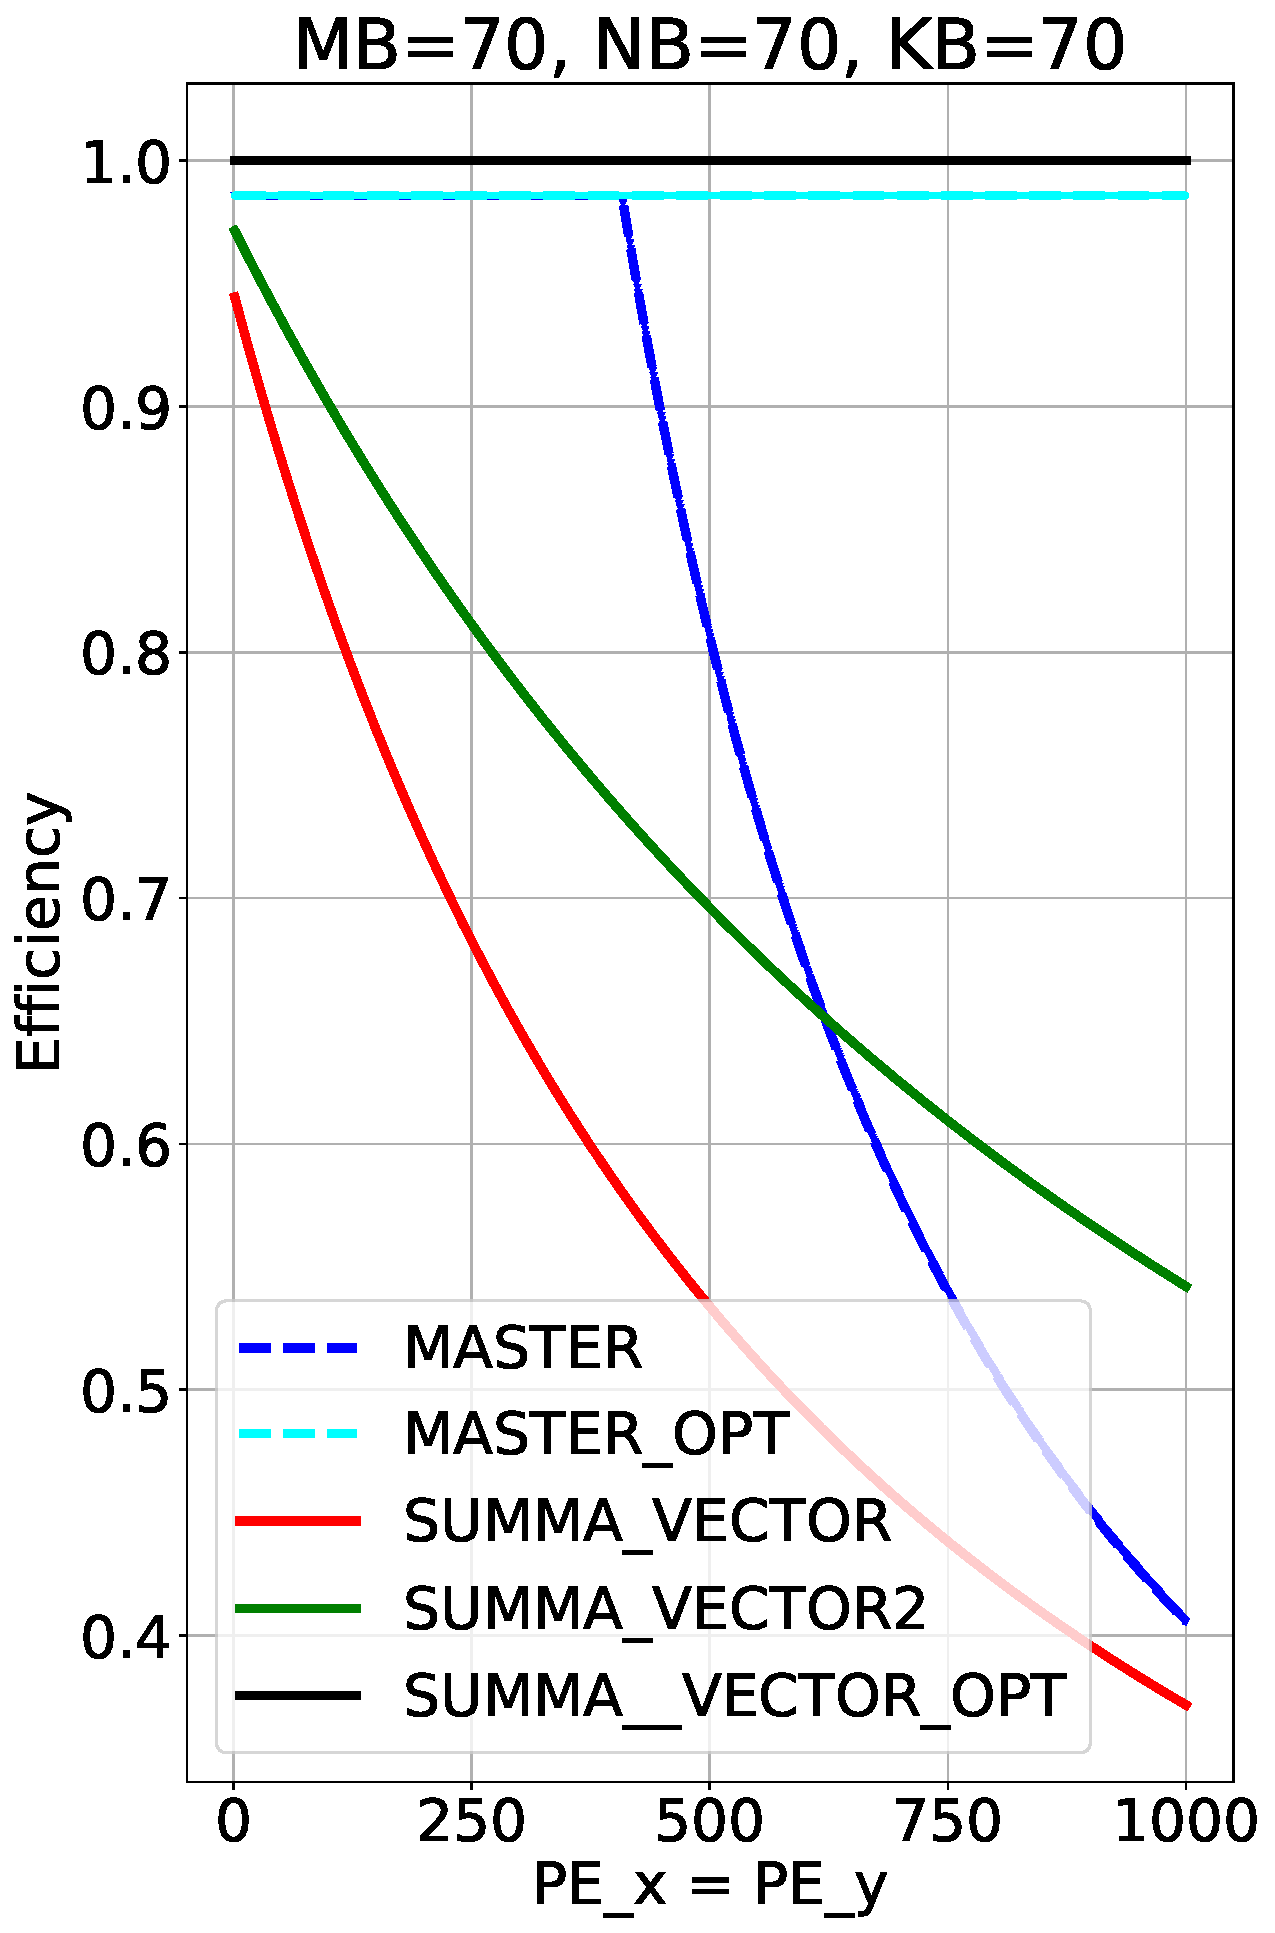
\includegraphics[width=\linewidth]{figures/efficiency_cost_70_70_70.pdf}
    %\caption{.}
    %\label{fig:gemm_master_1}
  \end{subfigure}
  \hfill
  %
  \begin{subfigure}{0.32\columnwidth}
    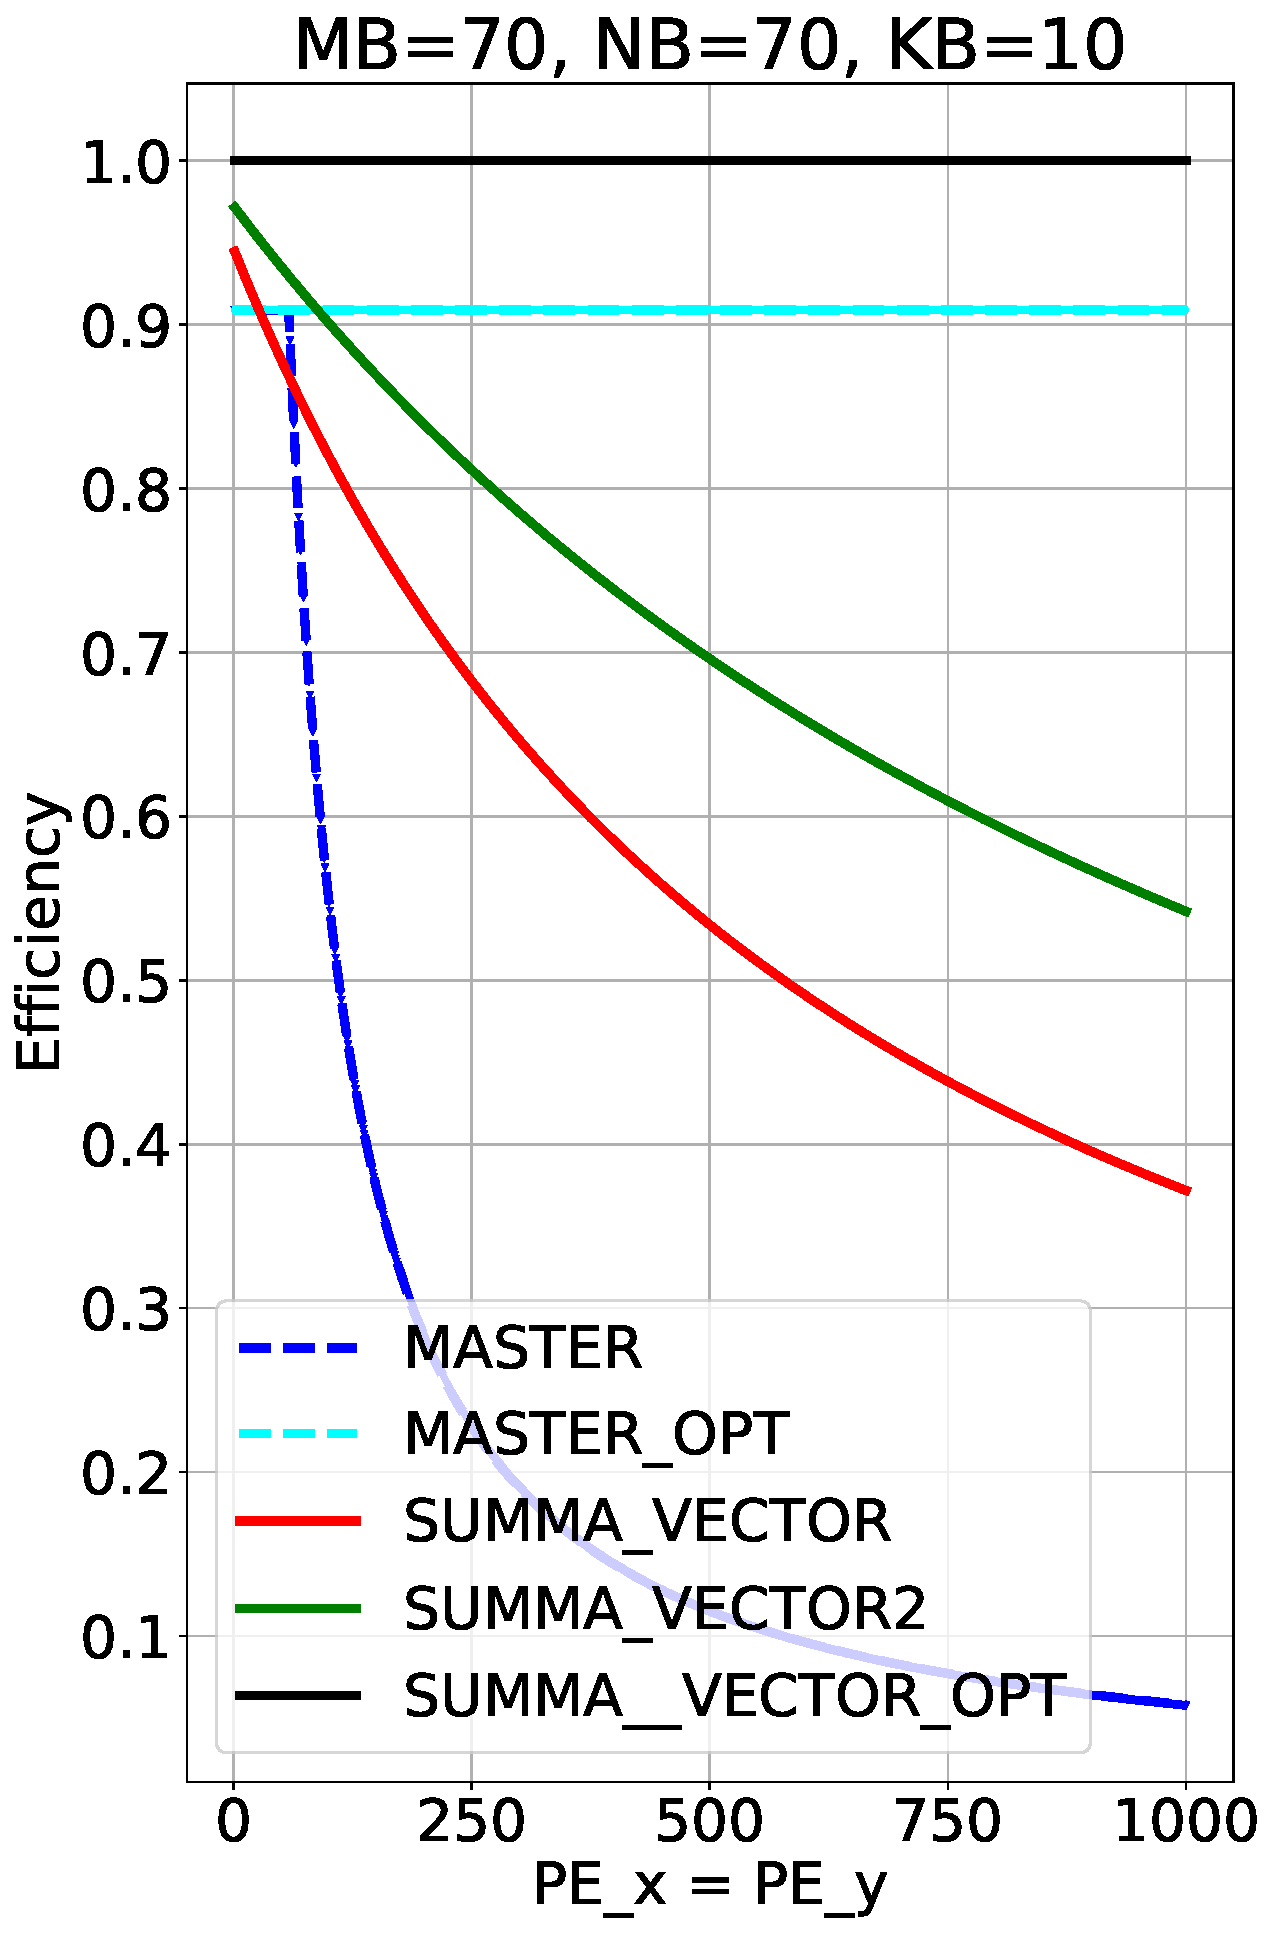
\includegraphics[width=\linewidth]{figures/efficiency_cost_70_70_10.pdf}
    %\caption{Non-ring.}
    %\label{fig:gemm_master_2}
  \end{subfigure}
  \hfill
  %
  \begin{subfigure}{0.32\columnwidth}
    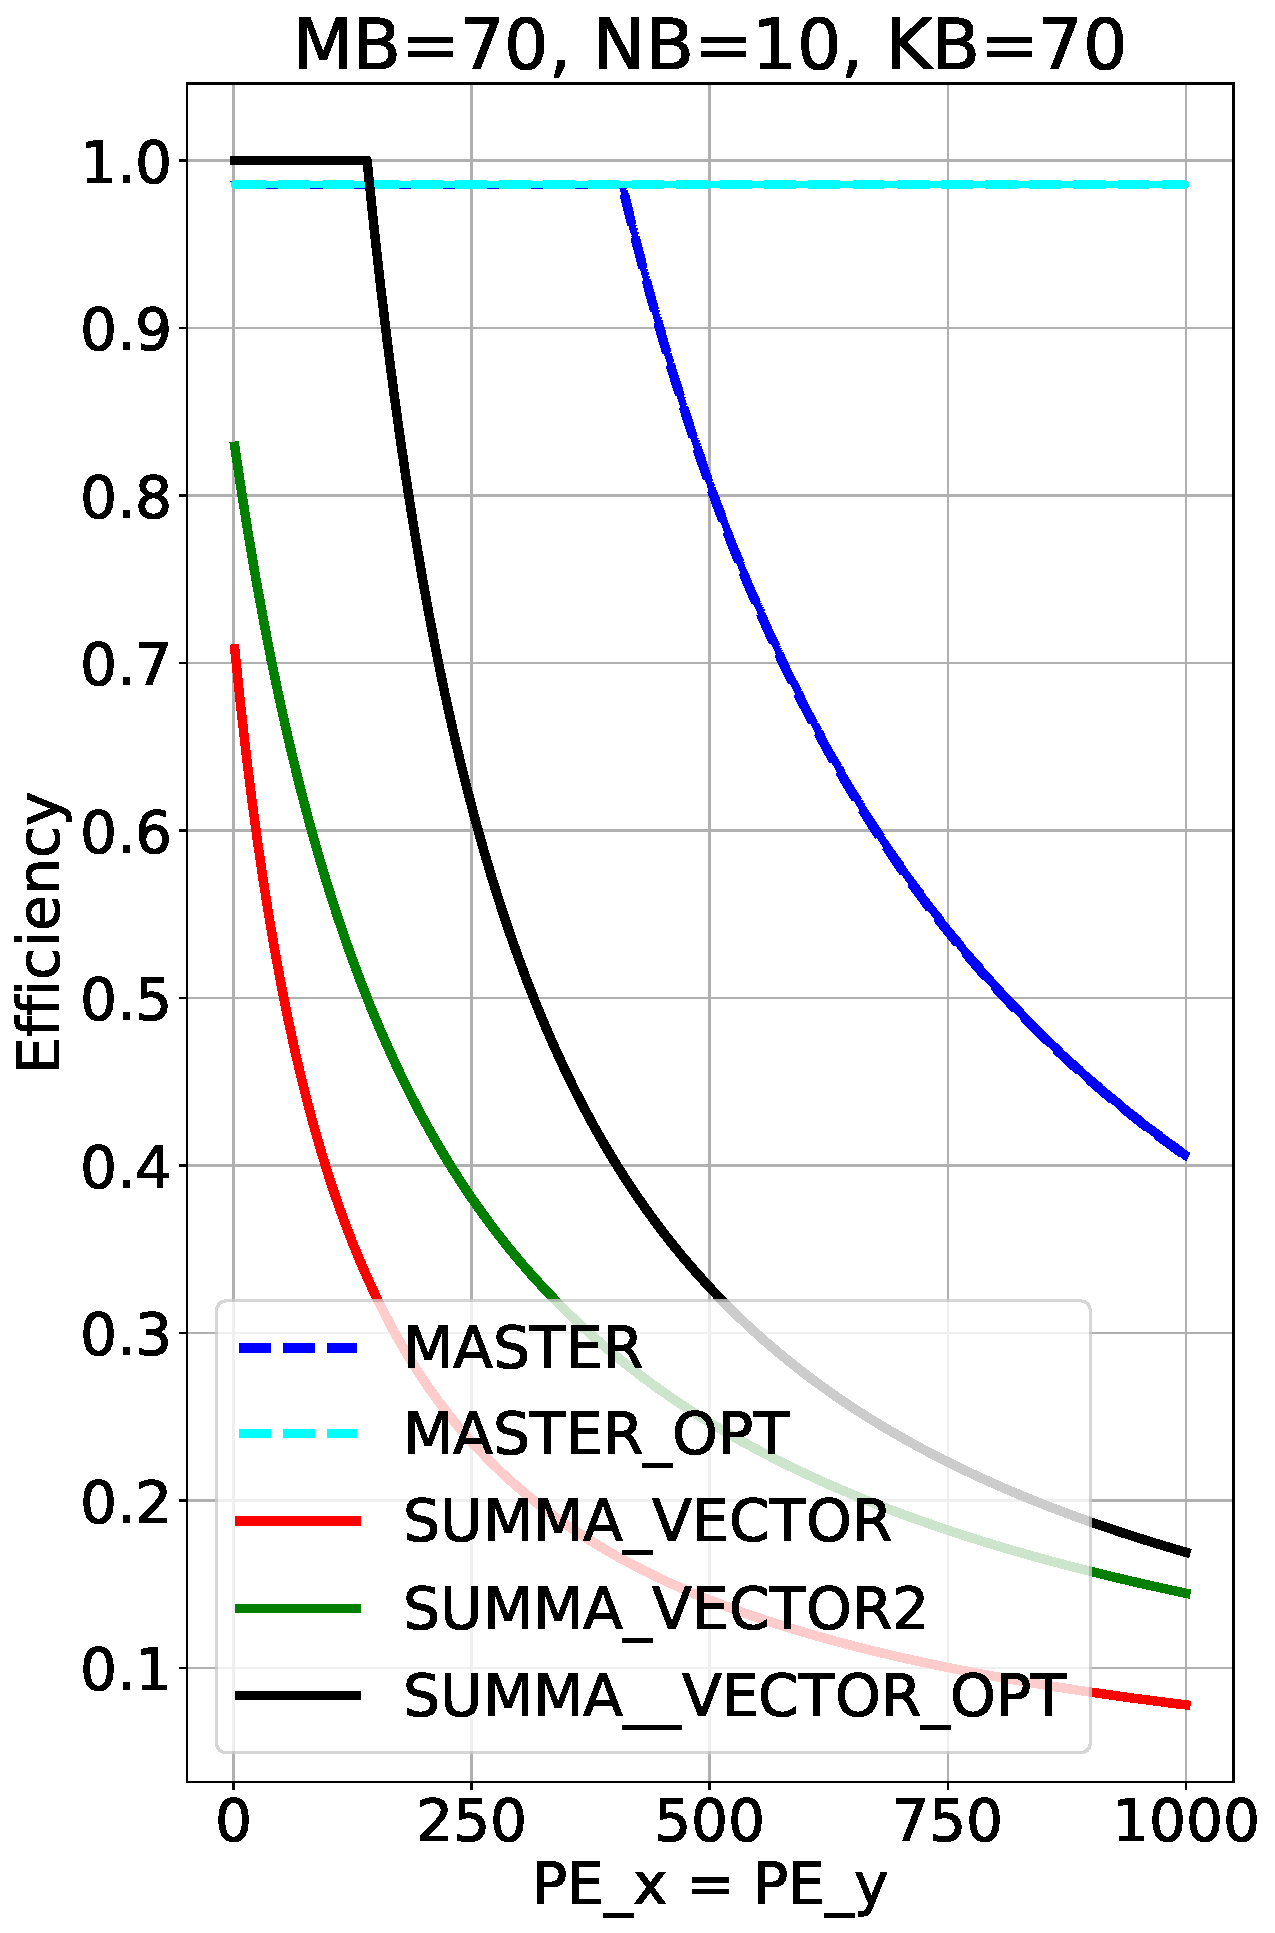
\includegraphics[width=\linewidth]{figures/efficiency_cost_70_10_70.pdf}
    %\caption{Non-ring.}
    %\label{fig:gemm_master_2}
  \end{subfigure}
  \caption{Performance simulation. ``MASTER": Equation~\ref{eq:master}; ``MASTER\_OPT": Equation~\ref{eq:master_2}; ``SUMMA\_VECTOR'': Equation~\ref{eq:summa_1}; ``SUMMA\_VERTOR2'': Equation~\ref{eq:summa_2}; ``SUMMA\_VECTOR\_OPT'': Equation~\ref{eq:summa_3}.}
  \label{fig:gemm_perf_simulate}
\end{figure}

Next, Table~\ref{table:exp_result} details some experimental and theoretical performance results.
%
Most of these experiments come from \texttt{test\_perf} in test\_matmul.
%
``Exp'' shorts for experimental, and ``Theo'' shorts for theoretical.
%
Numbers in bold are scenarios that \summa is better than \master.
%
From this table, we can see that 
\begin{itemize}
  \item the theoretical bound of \master possibly is between Equation~\ref{eq:master} and Equation~\ref{eq:master_2};
  \item the theoretical bound of \summa without optimization possibly is between Equation~\ref{eq:summa_1} and Equation~\ref{eq:summa_2};
  \item these results roughly follow the trends of their theoretical bounds.
\end{itemize}



\begin{table}[t!]
\caption{Performance results.}
%\footnotesize
\label{table:exp_result}
\centering
\begin{tabular}{cccc|ccc|cccc}
\toprule
\bf \makecell{K\\(hin)} & \bf \makecell{N\\(hout)} & \bf \makecell{M\\(batch)} & \bf \makecell{PE\_x\\(PE\_y)} & \bf \makecell{Exp\\ \master\\(cycles)} & \makecell{\bf Exp\\ \summa\\(cycles)} & \bf \makecell{Exp Ratio\\ \master/\summa} & \bf \makecell{Theo Eq\ref{eq:master}\\ \master\\ (cycles)}  & \bf \makecell{Theo Eq\ref{eq:master_2}\\ \master\\ (cycles)} & \bf \makecell{Theo Eq\ref{eq:summa_1}\\ \summa \\(cycles)} & \bf \makecell{Theo Eq\ref{eq:summa_2}\\ \summa \\(cycles)} \\
\midrule
128 & 128 & 128 & 16 & 5859 & 6946 & 0.84 & 6656 & 2352 & 7168 & 4608 \\
256 & 128 & 128 & 16 & 8874 & 13762 & 0.64 & 6656 & 4400 & 14336 & 9216 \\
128 & 256 & 128 & 16 & 11430 & 8996 & \bf 1.27 & 13312 & 4656 & 9216 & 7168 \\ 
256 & 256 & 128 & 16 & 17535 & 17863 & 0.98 & 13312 & 8752 & 18432 & 14336 \\
128 & 128 & 256 & 16 & 8002 & 10365 & 0.77 & 6912 & 4656 & 10240 & 7168 \\
256 & 128 & 256 & 16 & 12116 & 20626 & 0.58 & 8704 & 8752 & 20480 & 14336 \\
128 & 256 & 256 & 16 & 15803 & 14470 & \bf 1.09 & 13824 & 9264 & 14336 & 11264 \\
256 & 256 & 256 & 16 & 23982 & 28816 & 0.83 & 17408 & 17456 & 28672 & 22528 \\
128 & 128 & 384 & 16 & 10830 & 13875 & 0.78 & 7168 & 6960 & 13312 & 9728 \\
256 & 128 & 384 & 16 & 16969 & 27636 & 0.61 & 13056 & 13104 & 26624 & 19456 \\
128 & 256 & 384 & 16 & 21469 & 20022 & \bf 1.07 & 15872 & 13872 & 19456 & 15872 \\ 
256 & 256 & 384 & 16 & 33729 & 39924 & 0.84 & 26112 & 26160 & 38912 & 31744 \\
%10 & 10 & 10 & 10 & 348 & 293 & 1.18 & 325 & 212 & 107 \\
40 & 40 & 40 & 10 & 1289 & 1215 & \bf 1.06 & 1320 & 230 & 1120 & 640 \\ 
80 & 80 & 80 & 10 & 3636 & 3848 & 0.94 & 2720 & 1470 & 3520 & 2400 \\ 
720 & 20 & 720 & 10 & 27517 & 114820 & 0.23 & 26280 & 26310 & 92160 & 59040 \\
20 & 720 & 720 & 10 & 79132 & 28500 & \bf 2.77 & 38880 & 38910 & 27760 & 26840 \\ 

%\midrule
%Total & ${\frac{1}{3}} \times n^3$ & $$\\
%Total & & $O(N^2 \rank)$\\
\bottomrule
\end{tabular}
\end{table}


%\includegraphics{summa_gemm.gif}
